\chapter{尤度場モデルを使用したパーティクルフィルタ}
\section{はじめに}
本章では, 尤度場モデルを使用したパーティクルフィルタについて説明をする. 
尤度場モデルを使用したパーティクルフィルタは, 手持ちの地図から事前に求めた, 
マップ上の障害物検知の尤度を表すxy座標上の関数をパーティクルの尤度計算に使用して
自己位置を推定するアルゴリズム[\ref{alg:mcl}]である. 
この方法は, 得られるパーティクルの確率分布が雑然とした環境でも滑らかになることや尤度場の事前計算によって
計算効率の高いことがメリットとしてある. 

\begin{figure}[h]
  \begin{algorithm}[H]
      \caption{MCL($\mathcal{X}_{t-1}, u_t, z_t, m$)}
      \label{alg:mcl}
      \begin{algorithmic}
      \STATE $\mathcal{\bar{X}}_t = \mathcal{X}_t = 0$

      \FOR {$m = 1$ to $M$}
      \STATE $x_{t}^{[m]} = sample\_motion\_model(u_{t}, x_{t-1}^{[m]})$
      \STATE $w_{t}^{[m]} = likelihood\_field\_range\_finder\_model\_model(z_{t}, x_{t}^{[m]}, m)$
      \STATE $\mathcal{\bar{X}}_t = \mathcal{\bar{X}}_t + <x_{t}^{[m]}, w_{t}^{[m]}>$
      \ENDFOR

      \FOR {$m = 1$ to $M$}
      \STATE $draw\;i\;with\;probability \propto w_{t}^{[i]}$
      \STATE $add\; x_{t}^{[i]}\;to\;\mathcal{X}_t$
      \ENDFOR

      \RETURN $\mathcal{X}_t$
      \end{algorithmic}
  \end{algorithm}
  \caption{MCLの疑似コード}
\end{figure}

\section{パーティクルフィルタの目的・理論}

パーティクルフィルタは初期位置である$x_0$から, 入力される情報, 状態遷移モデル, 観測モデルを使用することで, 
確率密度関数である信念分布$b_t$を求め, パーティクルによる近似によって推定した自己位置である$x$を求めることを目的としている. 
$x$は$\sum_{world}$上でのロボットの位置を(x, y),向きを$\theta$で表した, 
式(\ref{exp:x})のようなロボットの姿勢である. 

\begin{eqnarray}
  \label{exp:x}
  x = (x, y ,\theta)^T
\end{eqnarray}

\subsection{自己位置推定における信念分布}

最初の姿勢を$x_0$, これまでの制御指令値を式(\ref{exp:u}), センサ値を式(\ref{exp:z})とした場合, 
推定したロボットの自己位置を表した信念分布$b_t$は式(\ref{exp:b_t})になる. 

\begin{eqnarray}
  \label{exp:u}
  u_{1:t} = \{u_t|t=1,2,3,...,t\} 
\end{eqnarray}

\begin{eqnarray}
  \label{exp:z}
  z_{1:t} = \{z_t|t=1,2,3,...,t\} 
\end{eqnarray}

\begin{eqnarray}
  \label{exp:b_t}
  b_t(x) = p_t(x|x_0, u_{1:t}, z_{1:t}) 
\end{eqnarray}
式(\ref{exp:b_t})の右辺から信念分布$b_t$を求めるためには状態遷移モデルである式(\ref{exp:u_m})と
観測モデルである式(\ref{exp:z_m})を用いる. 
しかし, 今回は尤度場モデルを使用するため, 式(\ref{exp:z_m})は式(\ref{exp:z_m_m})になる. 

\begin{eqnarray}
  \label{exp:u_m}
  x_t 〜 p(x|x_{t-1}, u_t)
\end{eqnarray}

\begin{eqnarray}
  \label{exp:z_m}
  z_t 〜 p(z|x_t)
\end{eqnarray}

\begin{eqnarray}
  \label{exp:z_m_m}
  z_t 〜 p(z|x_t, m)
\end{eqnarray}

\subsection{状態遷移モデルによる事前分布}

ロボットが時刻t-1からtまで, 制御指令値である$u_t$によって移動した場合, 
信念分布はロボットの姿勢と同様に$b_{t-1}$から遷移をする. 
遷移後の信念分布は式(\ref{exp:b_hat})である$\hat{b_t}$として表される. 

\begin{eqnarray}
  \label{exp:b_hat}
  \hat{b_t}(x) &=& p_t(x|x_0, u_{1:t}, z_{1:t-1}) \nonumber \\
  &=& \int_{x'\in\chi} p(x|x', u_t)b_{t-1}(x')dx' \nonumber \\
  &=& {<p(x|x', u_t)>}_{b_{t-1(x')}}
\end{eqnarray}

\subsection{観測更新による事後分布}

遷移後に観測$z_t$が得られた場合, ベイズの定理によって
信念分布$\hat{b_t}$の更新を行うことができる. 
更新後の信念分布は式(\ref{exp:b_beizu})で表された$b_t$になる. 

\begin{eqnarray}
  \label{exp:b_beizu}
  b_t(x) &=& \hat{b_t}(x|z_t, m) \nonumber \\
  &=& \frac{p(z_t|x, m)\hat{b_t}(x)}{p(z_t)} \nonumber \\
  &=& \eta p(z_t|x, m)\hat{b_t}(x)
\end{eqnarray}

\subsection{パーティクルによる近似}

信念分布$b_t$は$N$個のパーティクルによるパーティクルフィルタによって近似される. 
近似された信念分布$b_t$は, 式(\ref{exp:b_p})になる. 

\begin{eqnarray}
  \label{exp:b_p}
  P(x*\in X) &=& \int_{x'\in\chi}b_t(x)dx \nonumber \\
  &\approx& \frac{1}{N} \sum_{i=0}^{N-1} \delta (x^{(i)}_{t} \in X)
\end{eqnarray}

そして, 観測による更新を考慮すると, 式(\ref{exp:b_p})は
重み$w_t$によって式(\ref{exp:b_p_z})になる. 
Nはパーティクルの数である. 

\begin{eqnarray}
  \label{exp:b_p_z}
  P(x*\in X) &=& \int_{x'\in\chi}b_t(x)dx \nonumber \\
  &\approx& \sum_{i=0}^{N-1} w^{(i)}_{t} \delta (x^{(i)}_{t} \in X)
\end{eqnarray}
また, 観測値による重みは, 式(\ref{exp:b_p_w})のように尤度関数$L_j$から求められた
尤度に重みをかけることで求めることができる. 

\begin{eqnarray}
  \label{exp:b_p_w}
  w_{t}^{(i)} &=& L_j(x_{t}^{(i)} | z_{j, t}, m)\hat{w}_{t}^{i}
\end{eqnarray}

\subsection{リサンプリング}

観測による更新の後にパーティクルフィルタでは, 重みの偏りを防ぐために
パーティクルのリサンプリングを行う. リサンプリングは大きな重みを持ったパーティクル
をコピーしたものをその周辺にパーティクルを撒く. また, 小さな重みを持つパーティクルは
削除される. 

\section{課題点}

一般的なパーティクルフィルタは静的環境とマルコフ性を仮定しているという制限がある. 
なので, 動的障害物が常に観測情報として含まれている場合, 自己位置推定は影響を受け続ける. 
そういった影響に対応するために\cite{赤井2019}のようなアウトライヤーを棄却するアルゴリズムが
必要になってくる. 
しかし, 過度にアウトライヤーを棄却するとかえって自己位置推定に影響を与えてしまう. 
そのため, 自己位置推定に影響を与えずに尤度計算の前に観測情報の
アウトライヤーを棄却するようなアルゴリズムが必要である. (影響とは?)

\newpage
\section{パーティクルフィルタの流れ}
\begin{figure}[h]
  \begin{center}
    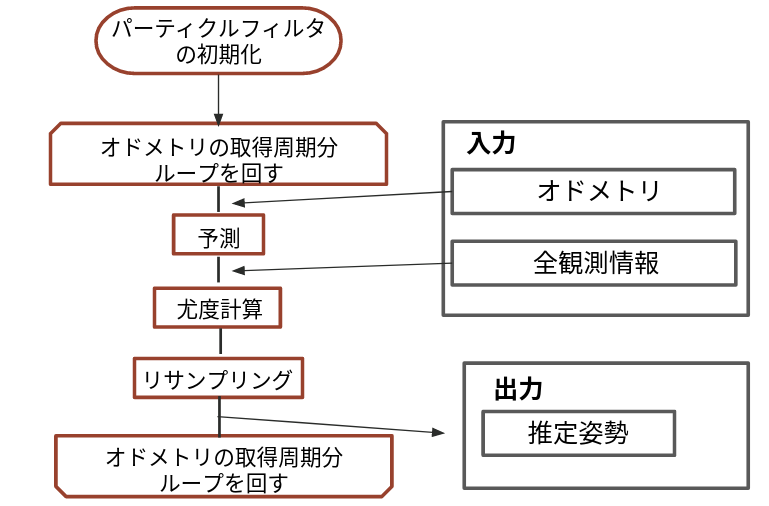
\includegraphics[width=1.2\linewidth]{figs/particle_filter_flow.png}
    \caption{パーティクルフィルタの流れ}
    \label{fig:particle_filter_flow}
  \end{center}
\end{figure}

\chapter{各パーティクルに観測範囲を付与した未知障害物対策}
\section{はじめに}
本章では, 提案手法である, 各パーティクルに観測範囲を付与することで未知障害物の対策をした, 
アルゴリズムについて説明する. 
このアルゴリズム[\ref{alg:proposed_mcl}]は, 各パーティクルに, 自己位置推定に影響を
与えないような観測範囲を与えることによって未知障害物の対応する
アルゴリズムである. 
また, 従来のパーティクルフィルタに対して, 
計算時間の増加なしに, 未知障害物による急激な尤度の低下を防ぐことができる. 

\begin{figure}[h]
  \begin{algorithm}[H]
      \caption{Proposed MCL($\mathcal{X}_{t-1}, u_t, z_t, m , p_{p\_\mathsf{angle}}$)}
      \label{alg:proposed_mcl}
      \begin{algorithmic}
      \STATE $\mathcal{\bar{X}}_t = \mathcal{X}_t = 0$

      \FOR {$p = 1$ to $P$}
      \STATE $x_{t}^{[p]} = sample\_motion\_model(u_{t}, x_{t-1}^{[p]})$
      \STATE $w_{t}^{[p]} = likelihood\_field\_range\_finder_model\_model(z_{t}, x_{t}^{[p]}, m, p_{p\_\mathsf{angle}})$
      \STATE $\mathcal{\bar{X}}_t = \mathcal{\bar{X}}_t + <x_{t}^{[p]}, w_{t}^{[p]}>$
      \ENDFOR

      \FOR {$p = 1$ to $P$}
      \STATE $draw\;i\;with\;probability \propto w_{t}^{[i]}$
      \STATE $add\; x_{t}^{[i]}\;to\;\mathcal{X}_t$
      \STATE $add\;\;p_{p\_\mathsf{angle}}\;to\;p$
      \STATE $\Uparrow サンプリングしたパーティクルにランダムな観測パターンを付与$
      \ENDFOR
      \FOR {$p = 1$ to $P$}
      \STATE $P_\mathsf{mode\_p\_\mathsf{angle}} \Leftarrow 全パーティクルの中で最瀕な観測パターン$
      \STATE $P_\mathsf{mode\_p\_\mathsf{angle}} = Mode\_p\_\mathsf{angle}(p\rightarrow p_{p\_\mathsf{angle}})$
      \ENDFOR
      
      \RETURN $\mathcal{X}_t, P_\mathsf{mode\_p\_\mathsf{angle}}$
      \end{algorithmic}
  \end{algorithm}
  \caption{提案した手法を用いたMCLの疑似コード}
\end{figure}

\subsection{パーティクルに観測パターンを付与}
まずはじめに, パーティクルフィルタはN個のパーティクルを生成する. 
次に, 未知障害物を観測した情報を棄却するために図\ref{fig:z_pattern}のような, 
観測パターンを用意する. そして, 生成された各観測パターンは, N個の各パーティクルに対して
ランダムに与えられる. その後は従来通り, 状態遷移モデルに従ってパーティクルをランダムに遷移させる. 

\newpage

\begin{figure}[H]
  \begin{center}
    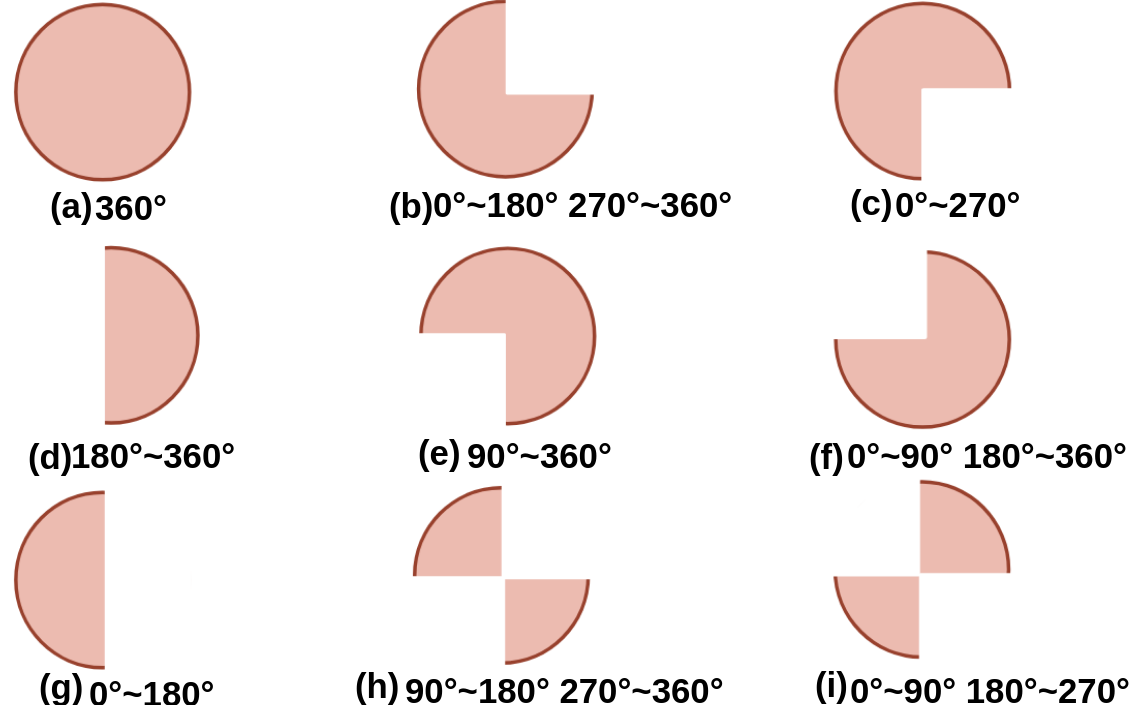
\includegraphics[width=0.8\linewidth]{figs/obs_pangle.png}
    \caption{観測パターン($p_\mathsf{angle}$)}
    \label{fig:1}
  \end{center}
\end{figure}

\subsection{尤度計算による観測パターンの評価}

遷移された各パーティクルの尤もらしさを評価するために尤度場を使用した尤度関数を用いて
各パーティクルの尤度を求める. 
観測パターンを持った各パーティクルの尤度は式[\ref{exp:b_p_w_angle}]のように求まる. 

\begin{eqnarray}
  \label{exp:b_p_w_angle}
  L_j(x_{t}^{(i)} | z_{j, t}, m, p_\mathsf{angle})
\end{eqnarray}
観測情報$z_t$を観測パターン$p_\mathsf{angle}$によってフィルタをかけることで, 使用する観測情報に制限をかけている. 
例えば, 図\ref{fig:z_pattern}のように, $p_\mathsf{angle} = (a)$を持ったパーティクルであれば, 
尤度計算に用いる観測情報は$z_t$の全てである. 
$p_\mathsf{angle} = (b)$を持ったパーティクルであれば, 尤度計算に用いる観測情報は$360°$のうち$0°〜90°$を間引いた
観測情報$z_t$になる. 


\subsection{リサンプリング時にランダムな観測パターンを付与}

パーティクルフィルタの初期化時に, 各パーティクルに与えた観測パターンのままであると, 
最尤なパーティクルの観測パターンを全てのパーティクル持つことになってしまう. 
つまり, ある観測パターンに収束したままになってしまい, 環境に応じて
観測パターンを変化させることができない状態に陥る. 
そのため, リサンプリング時にN個のパーティクルのうち$\frac{N}{10}$個程度のパーティクルをサンプリングし, 
ランダムな観測パターンを与える. 

\subsection{尤度計算とリサンプリングによる観測パターンの収束}

以上の尤度計算による観測パターンの評価とリサンプリングによるランダムな観測パターンを持ったパーティクルの
追加によって, パーティクルフィルタは環境に応じて, 適した観測パターンを各パーティクルに与えることができる. 
そして, 全パーティクルで最瀕な観測パターンを求めることで, 提案した手法を用いたパーティクルフィルタは, 
ロボットの姿勢と環境に適した観測パターンを求めることができる. 

\newpage
\section{提案した手法用いたパーティクルフィルタの流れ}

\begin{figure}[h]
  \begin{center}
    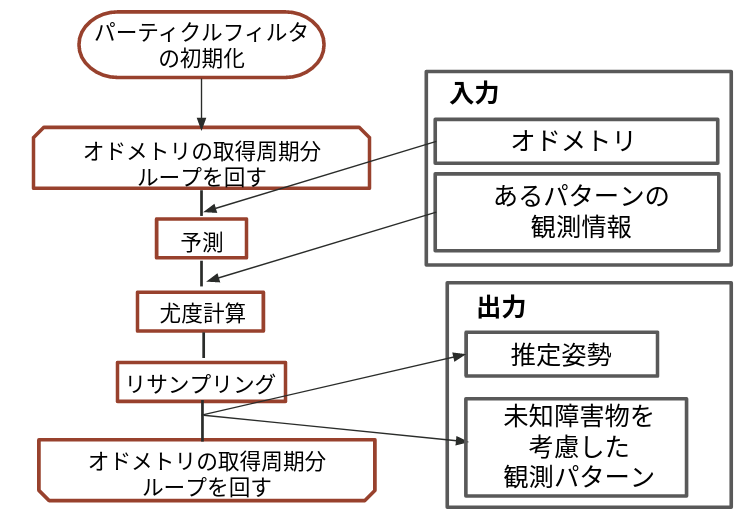
\includegraphics[width=1.0\linewidth]{figs/particle_filter_flow_improve.png}
    \caption{提案した手法用いたパーティクルフィルタの流れ}
    \label{fig:particle_filter_flow_improve}
  \end{center}
\end{figure}
